\chapter{Attacking CryptDB}
\label{chp:attacks}

In this chapter, a few known attacks on CryptDB will be presented along with the discussion around...

\section{Microsoft Research and their Frequency Analysis}

In September 2015, a Microsoft Research team released a paper stating that they had successfully broken the \gls{ope_onion} and the \gls{deterministic_onion} encryption schemes of CryptDB \cite{microsoft_cryptdb}. They did so by using one of the oldest tricks in a crypt analyst's book; frequency analysis.

\begin{wrapfigure}[13]{r}[1pt]{5.2cm}
\centering
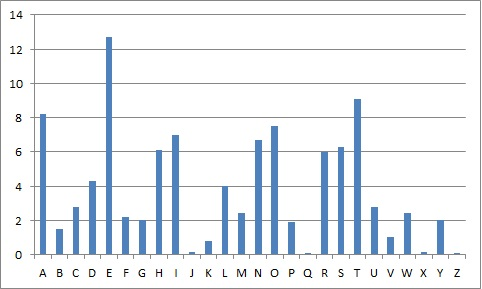
\includegraphics[scale=0.4]{letterfreq.jpg}
\caption{Bar chart of the letter frequency observed in the English language}
\label{fig:letter_freq}
\end{wrapfigure}
Frequency analysis is to exploit the fact that in most spoken languages, some characters and combinations of characters are more common than others. In the English alphabet, E, T, A and O are the most regular characters, while J, Z, Q and X are considered to be rare. As described in \ref{sec:det} and \ref{sec:ope}, the DET and OPE schemes are deterministic and therefore encrypts the same plaintext to the same ciphertext. \gls{ope_onion} also reveals the order between the ciphertexts. Because of this, an attacker with access to the ciphertexts is able to compute a histogram of the observed frequencies in the encrypted data. By comparing the histogram to a similar histogram of frequencies computed from closely related plaintext data, the attacker is able to determine which ciphertext characters corresponds to which plaintext characters with fairly large advantage.

% ???
As described in section \ref{sec:sqlaware}, in order for an application to be able to execute equality checks or order comparison, columns need to be encrypted with DET or OPE respectively. 




From an encrypted test database containing health records from multiple hospitals in the United States, Naveed, Kamara and Wright claimed to successfully have recovered 80\% of OPE-encrypted ciphertexts from 95\% of hospitals, and 60\% of DET-encrypted ciphertexts from 60\% of hospitals \cite{microsoft_cryptdb}. Their concrete attacks was a regular frequency analysis for attacking DET-encrypted columns along with a new attack called \emph{P-Optimization}. For decrypting OPE-encrypted columns, they used a regular sorting attack and a new cumulative sorting attack.

\subsection{Frequency Analysis on DET-encrypted Columns}

For decrypting DET-encrypted columns, frequency analysis was used where the $i$th most frequent element of an encrypted column $c$ was assigned to the $i$th most frequent element in an auxiliary dataset built with similar structured data. In addition to performing a plain frequency analysis, the researchs also presented a new attack called \emph{P-Optimization}. Instead of ordering frequencies from most frequent to less frequent, they find an allocation of ciphertext-plaintext pairs that minimizes the overall difference between the histogram computed by the frequency analysis and the auxiliary one. Finding the allocation that minimizes the difference in the histograms is formulated as \gls{lsap}, and can be solved by using a linear programming solver \cite{microsoft_cryptdb}.

For DET-encrypted columns, these attacks recovered the mortality risk and whether a patient lost its life while under hospital care for 100\% of the data items in 99\% and 100\% of the hospitals respectively. They also recovered 100\% of the data items in the column storing the severity of a disease for 51\% of the hospitals. Additionally to these columns, they also show that it is possible to decrypt some of the information related to race, sex, admission type, primary payer and major diagnostic category \cite{microsoft_cryptdb}.

\subsection{Sorting Attack on OPE-encrypted Columns}

When attacking columns encrypted using the OPE scheme, Microsoft Research used two approaches. The first approach was to use a sorting attack given that all of the columns where \emph{dense}. By dense, they mean that both the encrypted column and the equivalent column in the auxiliary dataset contains every element from the plaintext space. By sorting both values from the encrypted column and the auxiliary dataset and map the values based on rank, the attack is able to decrypt 100\% of the encrypted column. However, if the column does not contain all the possible plaintext from the plaintext space, the methodology has to be modified.

Cumulative attack for low-density columns is an approach where the attacker does not only leverage the scheme leaking the frequency of the ciphertexts, but also the relative ordering of the ciphertexts. If a ciphertext $c$ is greater than 90\% of the ciphertexts in the encrypted column, then it should be matched against values that are greater than 90\% of the elements in the plaintext space. By combing a \gls{cdf} and frequency analysis, and using an \gls{lsap} solver to find the most optimal pairing of ciphertexts and corresponding plaintexts, Microsoft Research was able to recover more than 80\% of encrypted data from 95\% of the hospitals \cite{microsoft_cryptdb}.

\subsection{CryptDB Developers Answer Microsoft Research}

In response to Microsoft Research's paper, the developers of CryptDB has presented a paper containing guidelines \cite{cryptdb_guidelines} on how to safely use CryptDB and remarks on where they claim Microsoft Research has used CryptDB in an unsafe way. One of the alleged flaws in the paper published by Microsoft Research was there inaccurate usage of the \gls{deterministic_onion} and \gls{ope_onion} schemes. As stated in section \ref{sec:sensitive}, sensitive data should be annotated using \verb!SENSITIVE! which ensures that the column is encrypted under a semantically secure encryption scheme such as \gls{random_onion}, \gls{hom_onion}, SEARCH or \gls{deterministic_onion} if the column has the unique constraint \cite{popa_thesis}. 

While Microsoft Research may have used CryptDB in an insecure way, it still addresses an interesting issue. Social security numbers, bank accounts, and such columns may be well suited for being marked as sensitive. But what about sensitive columns where one of the key features of the application is to perform order checks? For example in a medical system used at an emergency room, the doctors want to sort their patients based on the severity of their injuries and treat them accordingly. For this situation to work out in practice, the column has to be encrypted with \gls{ope_onion}, and therefore is vulnerable to the attacks presented above. After all, the main use of such systems as CryptDB is not to perform operations on non-sensitive data.